\documentclass[12pt,a4paper]{article}\usepackage[]{graphicx}\usepackage[]{xcolor}
% maxwidth is the original width if it is less than linewidth
% otherwise use linewidth (to make sure the graphics do not exceed the margin)
\makeatletter
\def\maxwidth{ %
  \ifdim\Gin@nat@width>\linewidth
    \linewidth
  \else
    \Gin@nat@width
  \fi
}
\makeatother

\definecolor{fgcolor}{rgb}{0.345, 0.345, 0.345}
\newcommand{\hlnum}[1]{\textcolor[rgb]{0.686,0.059,0.569}{#1}}%
\newcommand{\hlstr}[1]{\textcolor[rgb]{0.192,0.494,0.8}{#1}}%
\newcommand{\hlcom}[1]{\textcolor[rgb]{0.678,0.584,0.686}{\textit{#1}}}%
\newcommand{\hlopt}[1]{\textcolor[rgb]{0,0,0}{#1}}%
\newcommand{\hlstd}[1]{\textcolor[rgb]{0.345,0.345,0.345}{#1}}%
\newcommand{\hlkwa}[1]{\textcolor[rgb]{0.161,0.373,0.58}{\textbf{#1}}}%
\newcommand{\hlkwb}[1]{\textcolor[rgb]{0.69,0.353,0.396}{#1}}%
\newcommand{\hlkwc}[1]{\textcolor[rgb]{0.333,0.667,0.333}{#1}}%
\newcommand{\hlkwd}[1]{\textcolor[rgb]{0.737,0.353,0.396}{\textbf{#1}}}%
\let\hlipl\hlkwb

\usepackage{framed}
\makeatletter
\newenvironment{kframe}{%
 \def\at@end@of@kframe{}%
 \ifinner\ifhmode%
  \def\at@end@of@kframe{\end{minipage}}%
  \begin{minipage}{\columnwidth}%
 \fi\fi%
 \def\FrameCommand##1{\hskip\@totalleftmargin \hskip-\fboxsep
 \colorbox{shadecolor}{##1}\hskip-\fboxsep
     % There is no \\@totalrightmargin, so:
     \hskip-\linewidth \hskip-\@totalleftmargin \hskip\columnwidth}%
 \MakeFramed {\advance\hsize-\width
   \@totalleftmargin\z@ \linewidth\hsize
   \@setminipage}}%
 {\par\unskip\endMakeFramed%
 \at@end@of@kframe}
\makeatother

\definecolor{shadecolor}{rgb}{.97, .97, .97}
\definecolor{messagecolor}{rgb}{0, 0, 0}
\definecolor{warningcolor}{rgb}{1, 0, 1}
\definecolor{errorcolor}{rgb}{1, 0, 0}
\newenvironment{knitrout}{}{} % an empty environment to be redefined in TeX

\usepackage{alltt}
    \setlength\parindent{0pt}
    \usepackage{geometry}
    \usepackage{graphicx}
    \usepackage{grffile}
    \geometry{margin=0.5in}
\IfFileExists{upquote.sty}{\usepackage{upquote}}{}
\begin{document}

    \section*{Octopus}


    Species: \emph{Octopus vulgaris}, Stock code: 1-Western Coast 2-Bottom Trawl

Region: Iberia

Marine Ecoregion: Portugal

Reconstructed catch data used from years 1995 - 2021 

 For figure captions and method see http://www.seaaroundus.org/cmsy-method

    \begin{figure}[ht]
    \centering
    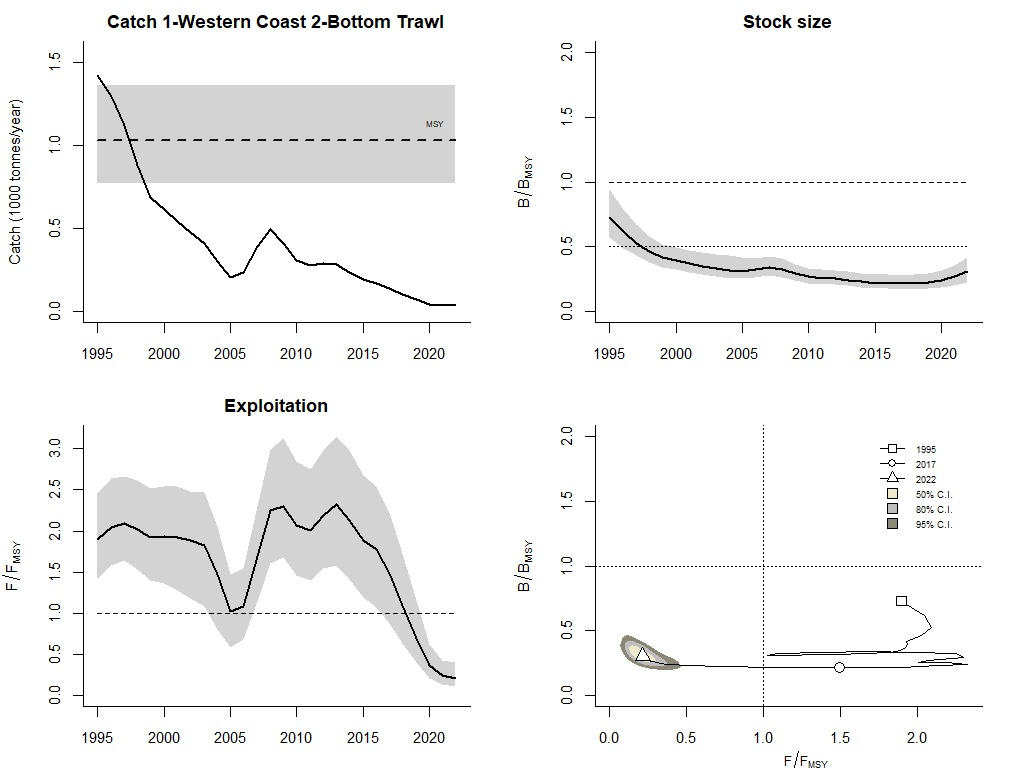
\includegraphics[width=1.00\textwidth ext=.jpg type=jpg]{1-Western Coast 2-Bottom Trawl_MAN.jpg}
    \end{figure}

    \textbf{Results for management (based on BSM analysis)}\\

Fmsy = 0.234, 95\% CL = 0.161 - 0.346 (if B $>$ 1/2 Bmsy then Fmsy = 0.5 r)

Fmsy = 0.149, 95\% CL = 0.102 - 0.22 (r and Fmsy are linearly reduced if B $<$ 1/2 Bmsy)

MSY = 0.975,  95\% CL = 0.735 - 1.3; Bmsy = 4.16,  95\% CL = 2.81 - 5.93 (1000 tonnes)

Biomass in last year = 1.32, 95\% CL = 0.848 - 1.99 (1000 tonnes)

B/Bmsy in last year = 0.317, 95\% CL = 0.23 - 0.439

Fishing mortality in last year = 0.0225, 95\% CL =0.0136 - 0.0374

F/Fmsy  = 0.151, 95\% CL = 0.0787 - 0.295 

 Comment:  

    \pagebreak

    \begin{figure}[ht]
    \centering
    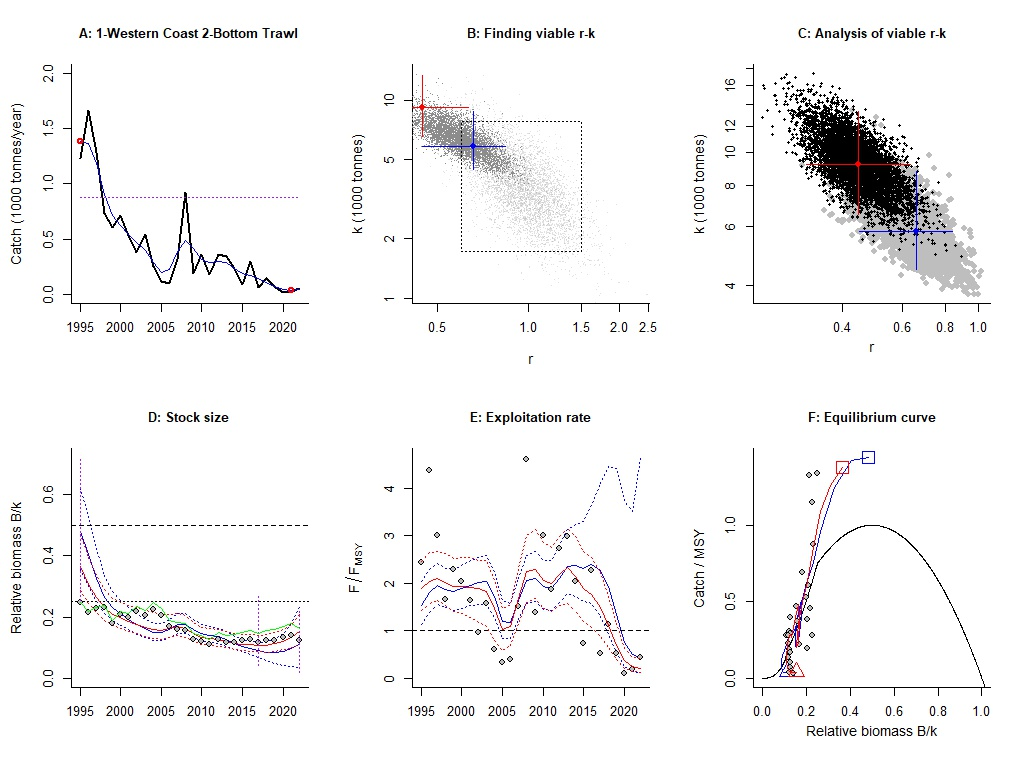
\includegraphics[width=1.00\textwidth ext=.jpg type=jpg]{1-Western Coast 2-Bottom Trawl_AN.jpg}
    \end{figure}

    \textbf{Results of CMSY analysis conducted in JAGS}\\

r = 0.659, 95\% CL = 0.456 - 0.841; k = 5.6, 95\% CL = 4.44 - 8.37 (1000 tonnes)

MSY = 0.923, 95\% CL = 0.713 - 1.21 (1000 tonnes/year)

Relative biomass last year = 0.0975 k, 95\% CL = 0.0267 - 0.222

Exploitation F/(r/2) in last year = 0.752 \\

\textbf{Results from Bayesian Schaefer model using catch and CPUE}\\

r = 0.468, 95\% CL = 0.322 - 0.692; k = 8.32, 95\% CL = 5.62 - 11.9

r-k log correlation = -0.719

MSY = 0.975, 95\% CL = 0.735 - 1.3 (1000 tonnes/year)

Relative biomass in last year = 0.0975 k, 95\% CL = 0.0267 - 0.222

Exploitation F/(r/2) in last year = 0.149

q = 3.92, 95\% CL = 2.74 - 5.78

Prior range of q = 1.04 - 18.3

Relative abundance data type = CPUE

Prior initial relative biomass = 0.256 - 0.721 default

Prior intermediate relative biomass = 0.0501 - 0.285 in year 2016 default

Prior final relative biomass = 0.0169 - 0.215, default

Prior range for r = 0.6 - 1.5 default, prior range for k = 1.77 - 7.77 (1000 tonnes) default

Source for relative biomass: 

DGRM

    \end{document}
